
\chapter{Capítulo}

\resumodocapitulo{Lorem ipsum dolor sit amet, consectetur adipiscing elit. Sed elementum
gravida risus non accumsan. Vivamus est magna, rhoncus a aliquam ut,
faucibus vitae ligula. Nam rhoncus dolor nec erat rhoncus eu sagittis
turpis ultrices. Quisque nisl neque, dictum ut congue eget, pellentesque
in felis. Pellentesque iaculis, quam eget rhoncus ultrices, augue
turpis malesuada ligula, nec dignissim metus lacus sed ligula. Duis
imperdiet risus eget nulla dictum non condimentum neque vestibulum.
Integer fringilla, nisl et viverra laoreet, arcu ante malesuada lorem,
vel ullamcorper odio orci eget eros. }

\section{Fundamentação }

Mauris viverra orci sit amet \citeauthor{article:dummy} mi varius at porta
felis volutpat. Aenean pharetra ultricies justo quis ultricies. Etiam
posuere gravida egestas. Nullam ac tortor in mi porta rutrum ac ac
tortor. Curabitur elit purus, cursus quis elementum tincidunt, facilisis
sit amet leo. Nam adipiscing eleifend ipsum, in viverra lorem luctus
rutrum. Donec vitae velit eros. Pellentesque habitant morbi tristique
senectus et netus et malesuada fames ac turpis egestas. Aliquam semper,
magna sed pulvinar blandit, sem ante eleifend nibh, et ultrices nisl
magna a urna. In fringilla, sapien aliquam dapibus vestibulum, nunc
orci commodo ipsum, vel rutrum tortor nulla vel mauris.

Another figure example:
\begin{figure}[H]
	\centering %
	\scriptsize %
	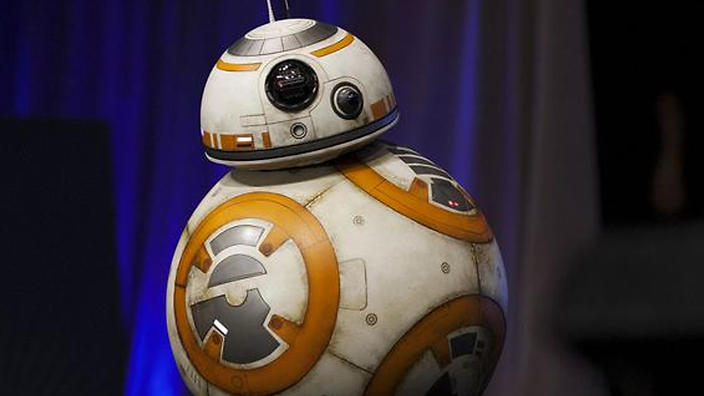
\includegraphics[width=\columnwidth]{new-bot}
	\caption{A new bot}
	\label{fig:new_bot}
\end{figure}

\section{Teoremas}

Maecenas nec orci at augue sollicitudin egestas. Suspendisse non risus
eget sapien sagittis ullamcorper ut at dolor. Class aptent taciti
sociosqu ad litora torquent per conubia nostra, per inceptos himenaeos.
Quisque a vestibulum augue. Donec erat mauris, molestie sed sagittis
sed, porttitor id elit. Nunc blandit accumsan lacus eu semper. Aliquam
cursus diam vel massa iaculis vitae laoreet tortor lacinia. Sed nibh
velit, dapibus et lacinia rutrum, rutrum id lorem. Aenean consectetur
accumsan elit, nec cursus dui commodo nec. Integer id elit vel mi
vulputate interdum sit amet sed tortor. Morbi auctor sem nec mauris
blandit eleifend. Aliquam erat volutpat. Donec mattis justo justo,
et condimentum lectus. Praesent suscipit arcu ac nunc pellentesque
consectetur.

Maecenas nec orci at augue sollicitudin egestas. Suspendisse non risus
eget sapien sagittis ullamcorper ut at dolor. Class aptent taciti
sociosqu ad litora torquent per conubia nostra, per inceptos himenaeos.
Quisque a vestibulum augue. Donec erat mauris, molestie sed sagittis
sed, porttitor id elit. Nunc blandit accumsan lacus eu semper. Aliquam
cursus diamd vel massa iaculis vitae laoreet tortor lacinia.
\begin{thm}[Título do Teorema (opcional)]
Dado X e Y, segue que 

\[
\int sss.
\]

Desta forma, o controlador é dado por $K=1$.
\end{thm}
\begin{proof}
Prova que X é igual a Y ou não

\[
\frac{d}{dt}1=0
\]

Segue, após algumas manipulações matemáticas, que X é igual a Y.
\end{proof}
Agora apenas para incluir um item de exemplo.
\begin{example}
Exemplo

Teste

Exemplo teste
\end{example}
Agora, veja como ficaria uma definição.
\begin{defn}
Definição XYZ

Seja XYZ, logo
\[
XYZ=XYZ.
\]
\end{defn}
A contagem dos Teoremas, Definições etc segue por capítulo e é independente
do 
\begin{thm}
Segue a descrição do novo teorema: 
\[
\int sss.
\]

Assim, está definido.

Por fim, observe como fica a chamada de Lemmas usando o template
\end{thm}
\begin{lem}[TESTE]
 Lema XYZ
\[
XYZ\iff xyz
\]
\end{lem}

